
\subsection{Text (GPT-4 \& Gemini): Chain-of-thought with the effect of delineation on accuracy}

\begin{itemize}
    \item Prompt Engineering Type Tested:  One-/Few Shot Prompting
    \item What are the 'ground truth' values: Human-Validated Finalised Orders.
    \item Evaluation Metric: Accuracy/F1 + Confusion Matrix.
\end{itemize}

Chain-of-thought encourages LLMs to mimic the reasoning  process of a human within the LLM by asking it to break the problem down into smaller problems.  Typically, with the Chain-of-thought reasoning approach, the output of the text is verbose as each chain of the thought process is reported, which means statistical comparison with other outputs is cumbersome due to its nondeterministic nature (see Figure \ref{fig:c-o-t-prompt} and \ref{fig:c-o-t-response}).In prompt engineering, the delimitation describes the expected output of the return response from an LLMs. Delineation allows us to test other prompt engineering techniques, such as chain-of-thought (see Figure \ref{fig:c-o-t-delin} and \ref{fig:c-o-t-delin-response}).

\begin{figure}
    \centering
    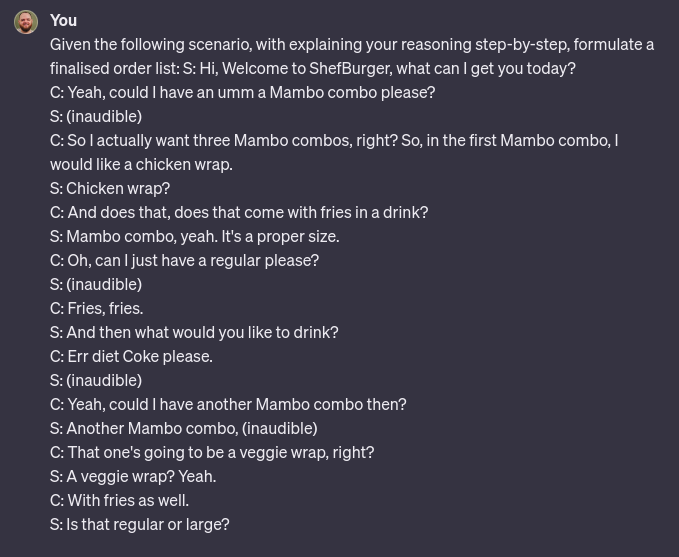
\includegraphics[width=1\linewidth]{sections//images/cot_no_delineation.png}
    \caption{Example input for chain-of-thought prompt engineering with no delineation}
    \label{fig:c-o-t-prompt}
\end{figure}

\begin{figure}
    \centering
    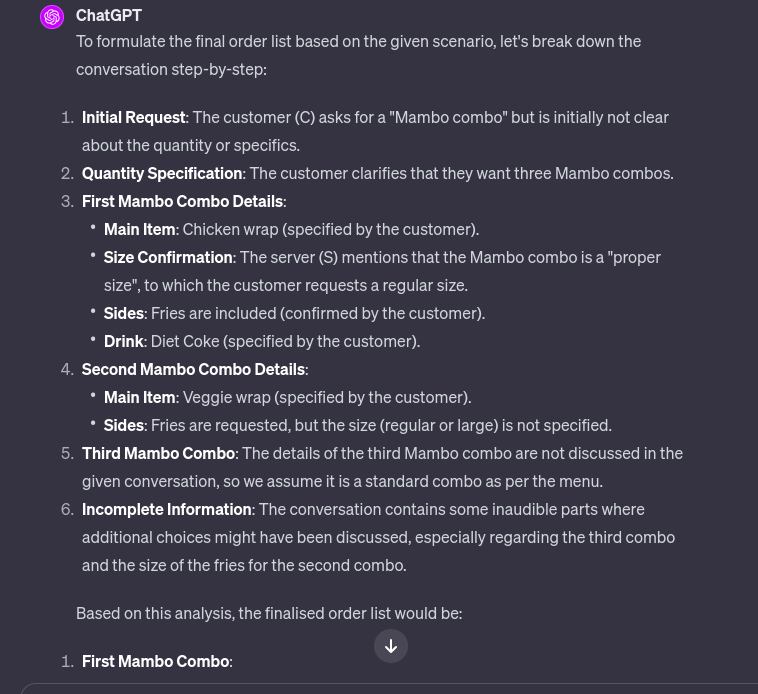
\includegraphics[width=1\linewidth]{sections//images/cot_no_delineation_response.png}
    \caption{Example response for chain-of-thought prompt engineering with no delineation}
    \label{fig:c-o-t-response}
\end{figure}

\begin{figure}
    \centering
    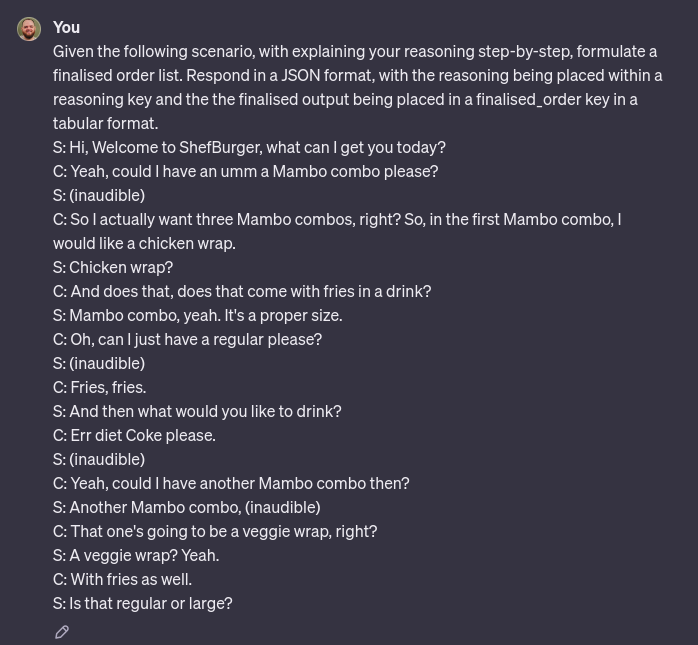
\includegraphics[width=1\linewidth]{sections//images/cot_with_delineation.png}
    \caption{Example input for chain-of-thought prompt engineering with delineation}
    \label{fig:c-o-t-delin}
\end{figure}

\begin{figure}
    \centering
    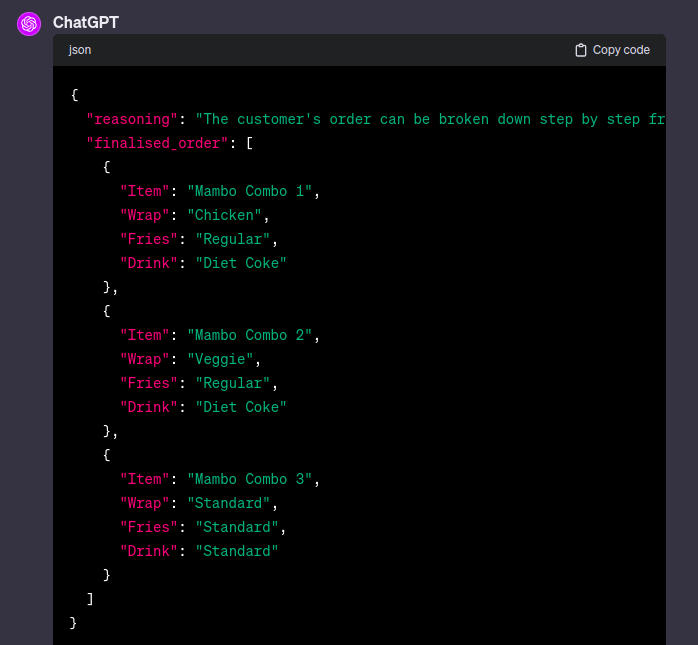
\includegraphics[width=1\linewidth]{sections//images/cot_with_delineation_response.png}
    \caption{Example response for chain-of-thought prompt engineering with delineation}
    \label{fig:c-o-t-delin-response}
\end{figure}